\section{Previous Semester}
\begin{frame}
     \begin{center}
     	\huge Previous Semester
     \end{center}
\end{frame}

\begin{frame}
\frametitle{Previous Semester}
\begin{center}
\textit{How can recommendations be made to a group of people by reflecting a groups decision making process, ensuring a high level of satisfaction in the group?}
\end{center}

Working with the assumption that Borda Count was a good mediator but could be improved

\begin{itemize}
\item Borda Transferable Count - Mix of Borda Count and Single Transferable Vote
\item Borda Escalating Count - Having a multiplication factor depending on the item rank
\item Borda Weighted Count - Gets assigned additional points based on the amount if lists an item occurs on
\end{itemize}
\end{frame}

\begin{frame}
\frametitle{Thesis Questions}
\begin{itemize}
\item How does Borda Count perform compared to state-for-the-art rank aggregation methods?
\item How does Borda Count perform on a dataset for group recommendation?
\item How does rearranging top-k lists influence the groups satisfaction?
\end{itemize}
\end{frame}

\section{Current Semester}
\begin{frame}
     \begin{center}
     	\huge Current Semester
     \end{center}
\end{frame}

\begin{frame}
\frametitle{Group Recommendation System}
\begin{columns}
	\begin{column}{0.55\textwidth}
		Individual Recommendations
		\begin{itemize}
			\small
			\item Trained matrix with the predicted individual ratings
			\normalsize
		\end{itemize}
		Groups
		\begin{itemize}
			\small
			\item Artificial constructed groups used for testing
			\normalsize
		\end{itemize}
		Group Recommendation
		\begin{itemize}
			\item Preprocessing 
			\begin{itemize}
				\item Formatting individual lists into ranked top-k lists
			\end{itemize}
			\item Rank aggregation 
			\begin{itemize}
				\item Performing the aggregation and returns the recommendations
			\end{itemize}
		\end{itemize}
		Evaluation
		\begin{itemize}
			\small
			\item An extensive test setup for the evaluation
			\normalsize
		\end{itemize}
	\end{column}
	\begin{column}{0.45\textwidth}
		\begin{figure}
			\centering
			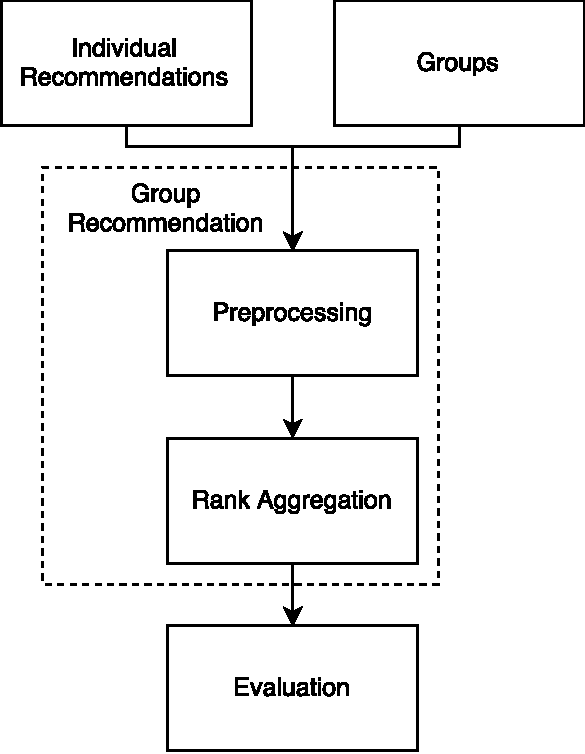
\includegraphics[scale=.5]{graphics/composition}
		\end{figure}
	\end{column}
\end{columns}
\end{frame}

\begin{frame}
\frametitle{Alternative Aggregation Methods}
\begin{columns}
	\begin{column}{0.5\textwidth}
		Voting systems
		\begin{itemize}
			\item Borda Count
		\end{itemize}
		Graph based methods
		\begin{itemize}
			\item Markov Chain 
			\item Spearman's Footrule
				\begin{itemize}
				\item $P = \{1, ..., |I|\}$
				\end{itemize}
			\begin{align*}
			W(i,p) = \displaystyle\sum_{n=1}^{u} |\frac{\tau_n(i)}{k} - \frac{p}{k}|
			\end{align*}
		\end{itemize}
		Others
		\begin{itemize}
			\item Average
		\end{itemize}
	\end{column}
	\begin{column}{0.5\textwidth}
		\begin{figure}
			\centering
			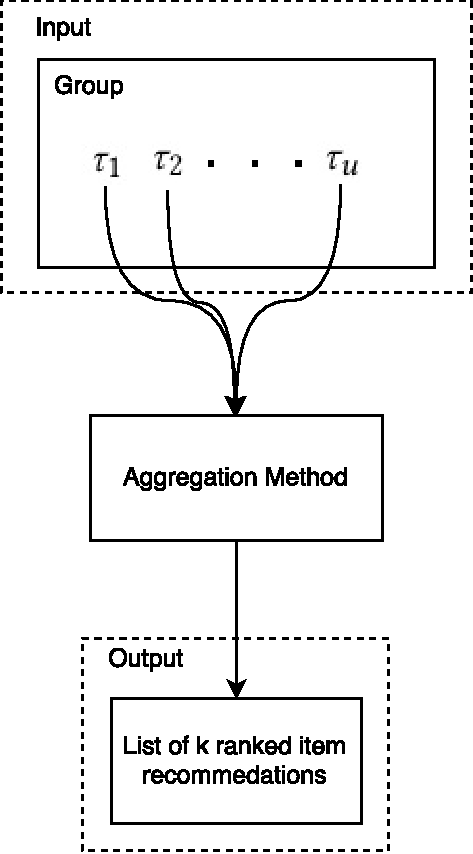
\includegraphics[scale=.4]{graphics/setuptransposed}
		\end{figure}
	\end{column}
\end{columns}
\end{frame}

%\begin{frame}
%\frametitle{Aggregation Methods}
%
%\end{frame}